\section{Implementation}

In this section we will discuss the implementation of the beer information retrieval system, focusing on the main components of the system and the technologies used to build them.

The information retrieval system is composed of two main components: the backend and the frontend. In the following subsections both components will be described in detail to give a better understanding of the inner workings of the system.


\subsection{Backend}

The backend is the core of the system as it is responsible for the business logic of the system.

The backend offers two main functionalities: indexing the dataset leveraging \textit{PyTerrier}, and a set of \textit{REST APIs} to query the index and retrieve the results in JSON format and to perform relevance feedback.

It is built using \textit{Python} and \textit{FastAPI}, a modern, fast (high-performance), web framework for building APIs. This particular framework has been chosen because it is easy to use, it is well documented and allows to build APIs in a matter of minutes.

\subsubsection{Endpoints}

Two REST API endpoints are offered by the backend:

\begin{enumerate}
  \item \texttt{/search} is the endpoint used to perform a query to the index. It accepts a \texttt{GET} request with the following query parameters:

        \begin{itemize}
          \item \texttt{query}: the query to be performed to the index.
          \item \texttt{top}: the number of results to be returned.
        \end{itemize}

        Example of a request to the \texttt{/search} endpoint:

        \begin{lstlisting}[language=bash]
      curl -X 'GET' \
        'http://localhost:8000/search?query=ipa&top=10' \
        -H 'accept: application/json'
    \end{lstlisting}

  \item \texttt{/feedback} is the endpoint used to perform relevance feedback. It accepts a \texttt{POST} request with the following body parameters:

        \begin{itemize}
          \item \texttt{query}: the query to be performed to the index.
          \item \texttt{relevant}: the list of document IDs that the user considers relevant.
          \item \texttt{irrelevant}: the list of document IDs that the user considers irrelevant.
        \end{itemize}

        Additionally, the \texttt{top} query parameter can be specified to control the number of results to be returned.

        Example of a request to the \texttt{/feedback} endpoint:

        \begin{lstlisting}[language=bash]
        curl -X 'POST' \
          'http://localhost:8000/feedback?top=10' \
          -H 'accept: application/json' \
          -H 'Content-Type: application/json' \
          -d '{
            "query": "ipa",
            "relevant": [
              "d1",
              "d2"
            ],
            "irrelevant": [
              "d3",
              "d4"
            ]
          }'
        \end{lstlisting}
\end{enumerate}

The documentation of the endpoints is automatically generated by \textit{FastAPI} and can be accessed at \texttt{http://localhost:8000/docs}. From this page it is possible to interact with the endpoints and test them in real-time directly from the browser.

\subsubsection{Commands}

To offer simple commands to interact with the backend, a \textit{Makefile} is provided. The commands are:

\begin{itemize}
  \item \texttt{make build-index} builds the reverse index from the dataset crawled from the web (refer to Section \ref{sec:data-scraping} for more details).
  \item \texttt{make dev} starts the backend in development mode, which means that the server will automatically restart when a change in the code is detected.
  \item \texttt{make start} starts the backend in production mode.
\end{itemize}

\subsection{Frontend}

The frontend allow users to interact with the search engine in a more user-friendly way. As already cited in the introduction present at the beginning of this report, the frontend is built using cutting-edge technologies:

\begin{itemize}
  \item \textit{TypeScript} is a programming language developed by Microsoft. It is a superset of JavaScript that adds static typing to the language. It is a very powerful language that allows to build complex web applications.

  \item \textit{NextJS} is a framework built on top of \textit{React.js} that allows to build server-side rendered web applications. It is a very powerful framework that allows to build web applications in a matter of minutes.

  \item \textit{React.js} is a JavaScript library for building user interfaces. It is a very popular library that is used by many companies to build their web applications.

  \item \textit{Chakra UI} is a component library that provides a set of accessible and reusable components that can be used to build user interfaces.
\end{itemize}

The frontend is composed of two main pages: a homepage that allows the user to perform an initial search (refer to Figure \ref{fig:home-page}), and a search page that allows the user to visualize, filter and sort the results of the query (refer to Figure \ref{fig:seach-page}). Additionally, this last page allows the user to perform relevance feedback to improve the results of the given query.

% Home page screenshot
\begin{figure}[H]
  \centering
  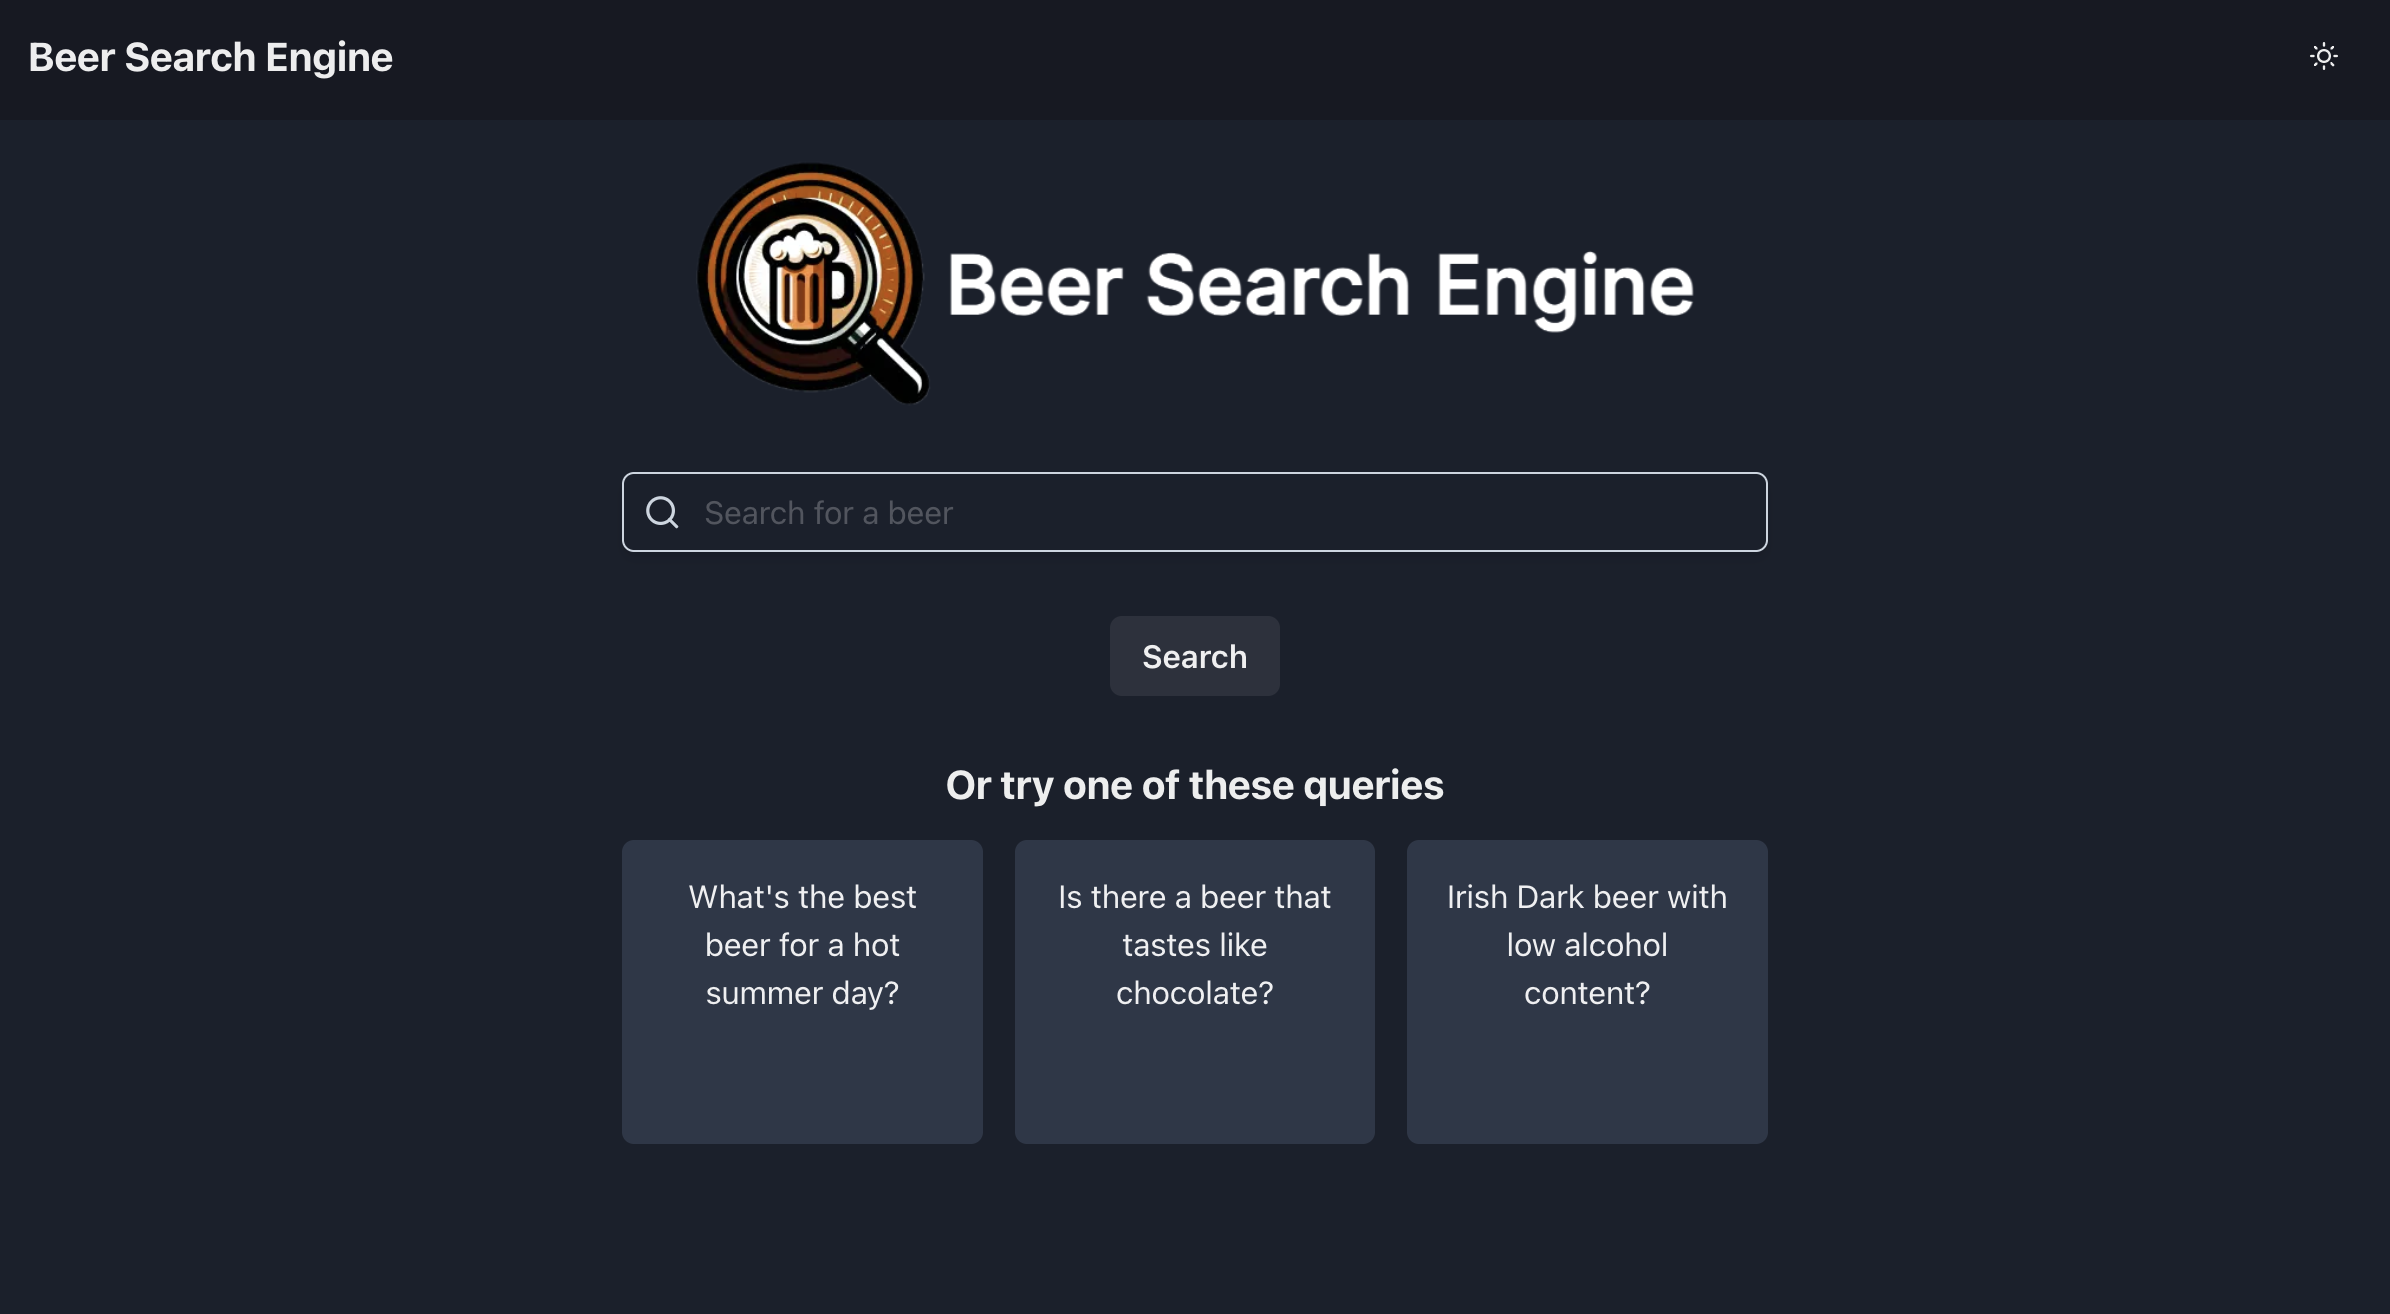
\includegraphics[width=1\textwidth]{img/3_implementation/homepage.png}
  \caption{Web interface homepage that allows the user to perform an initial search.}
  \label{fig:home-page}
\end{figure}

% Search page screenshot
\begin{figure}[H]
  \centering
  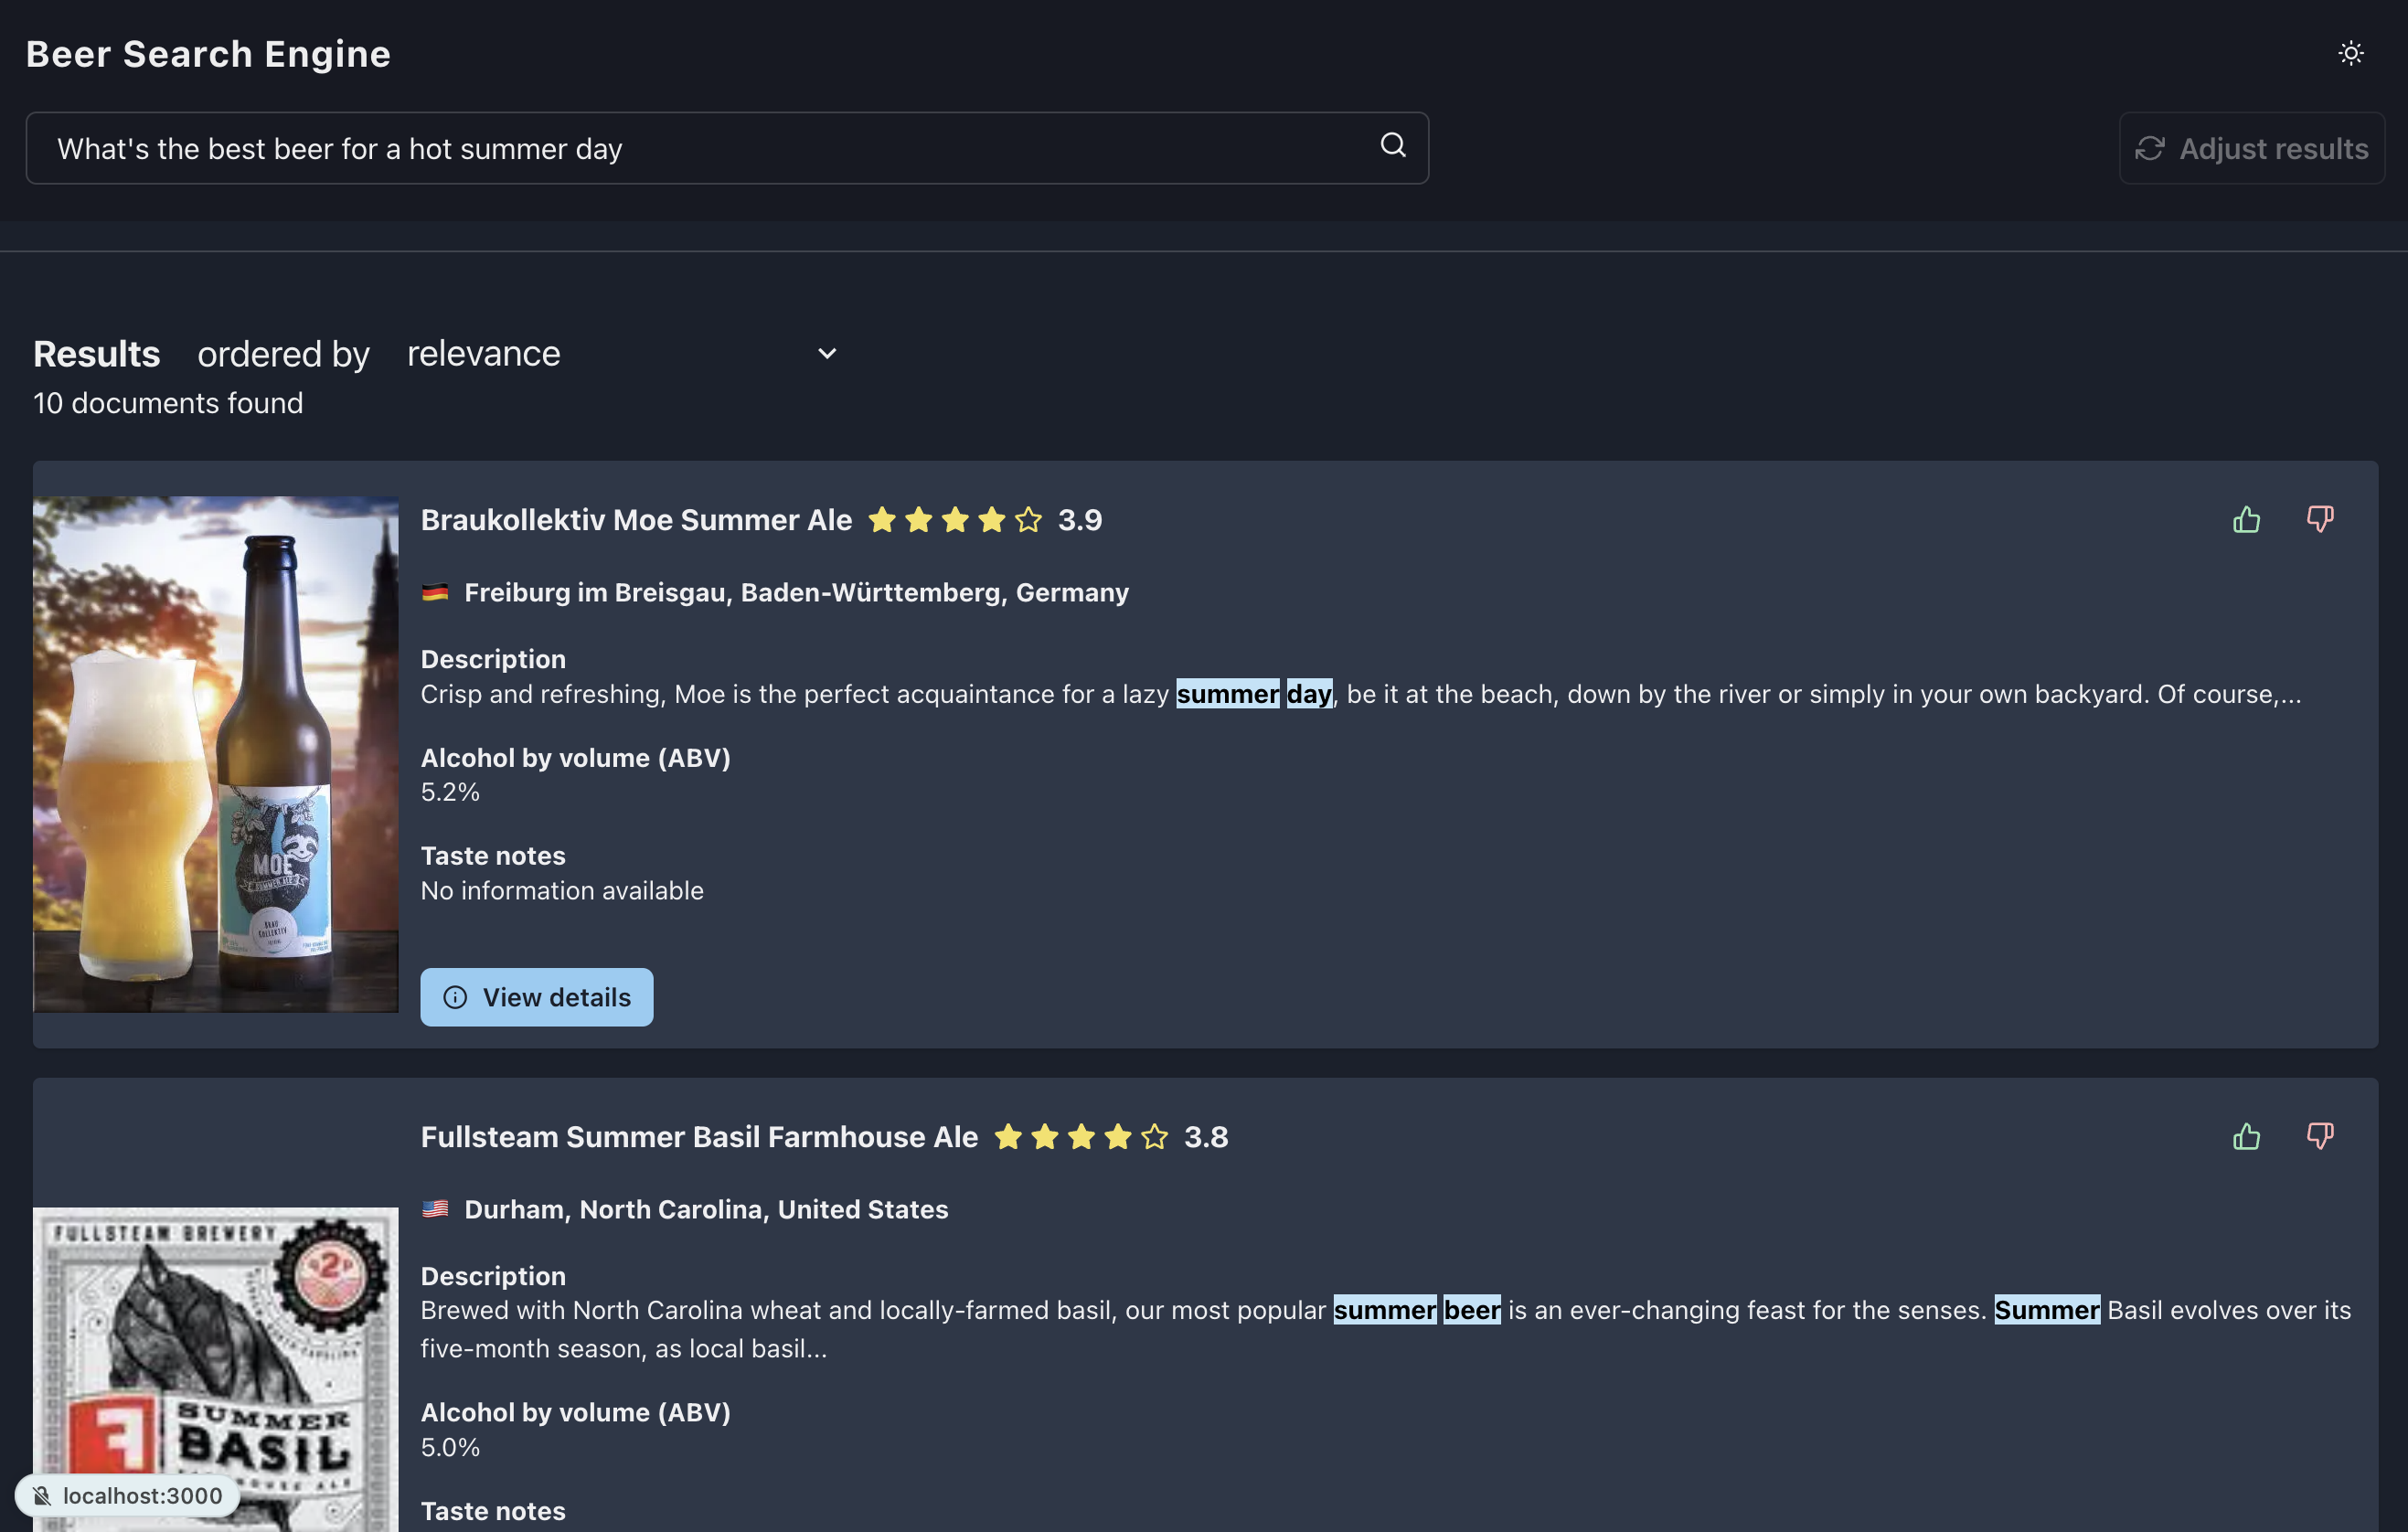
\includegraphics[width=1\textwidth]{img/3_implementation/search-page.png}
  \caption{Search page that allows the user to visualize the query results and perform relevance feedback on them to improve the results.}
  \label{fig:seach-page}
\end{figure}

\subsubsection{Features}

The frontend offers the following features:

\begin{itemize}
  \item Simple and intuitive user interface that allows the user to perform a search in a matter of seconds.
  \item The user can perform relevance feedback to improve the results of the query.
  \item The user can filter the results by multiple criteria: relevance (default), ABV (Alcohol By Volume), rating and name, allowing also to sort the results by ascending or descending order.
  \item Result snippets are provided to give the user a better understanding of why a result is relevant to the query by highlighting the present query terms.
  \item The entire interface supports both light and dark mode.
  \item Has been put a strong focus on accessibility, supporting screen readers and choosing colors that are accessible to visually impaired users (refer to Section \ref{sec:lighthouse-benchmark} for more details).
\end{itemize}

\subsubsection{Lighthouse benchmark}
\label{sec:lighthouse-benchmark}

\newpage
\subsection{Flow of execution}

To allow readers to better understand the flow of execution of the system, Figure \ref{fig:flow-diagram} outlines the main steps that are performed when a user performs a search and relevance feedback.

% Flow diagram of the system
\begin{figure}[H]
  \centering
  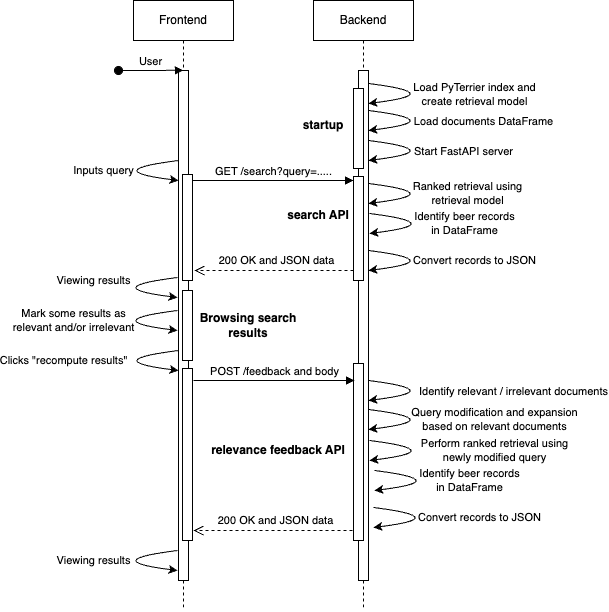
\includegraphics[width=1\textwidth]{img/3_implementation/search-flow.png}
  \caption{Flow diagram describing the execution of the system when a user performs a search and relevance feedback.}
  \label{fig:flow-diagram}
\end{figure}
\newpage


\subsection{Deployment}